\section{Ergebnisse}

\begin{table*}
	\caption{Numerische Auflistung der Ergebnisse der Frage 'Please enter your age in years'.}~\label{tab:sc_results_gender}
	
	\setlength\tabcolsep{3pt}
	\renewcommand{\arraystretch}{1.4}% for the vertical padding
	\begin{tabularx}{\textwidth}{ | x || r | r | }
		\hline
		Geschlecht & Absolutwerte 	& Prozentwerte \\ \hline\hline
		Männlich & 33 & 73.3\% \\ \hline
		Weiblich & 12 & 26.7\% \\ \hline
		Divers & 0 & 0.0\% \\ \hline
	\end{tabularx}
\end{table*}

\begin{figure}
	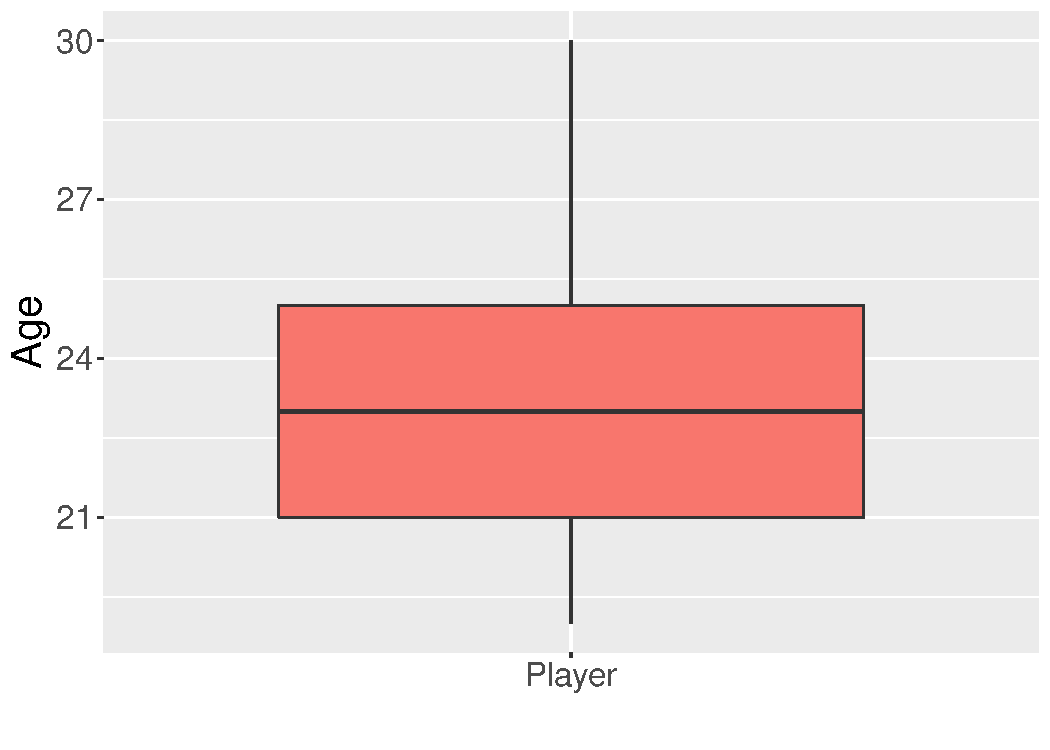
\includegraphics[width=\textwidth]{./appendices/age}
	\caption{Boxplot des Alters der Studienteilnehmer}
	\label{fig:age}
\end{figure}

\begin{table*}
	\caption{Numerische Auflistung der Ergebnisse der Frage 'Please select your gender'.}~\label{tab:sc_results_age}
	
	\setlength\tabcolsep{3pt}
	\renewcommand{\arraystretch}{1.4}% for the vertical padding
	\begin{tabularx}{\textwidth}{ | x | x | x | x | x | x | }
		\hline
		Min & Max & Range & Median & Mean  & Standard Deviation \\ \hline\hline
		19  & 30  & 11    & 23     & 23.04 & 2.53              \\ \hline
	\end{tabularx}
\end{table*}

\begin{figure}
	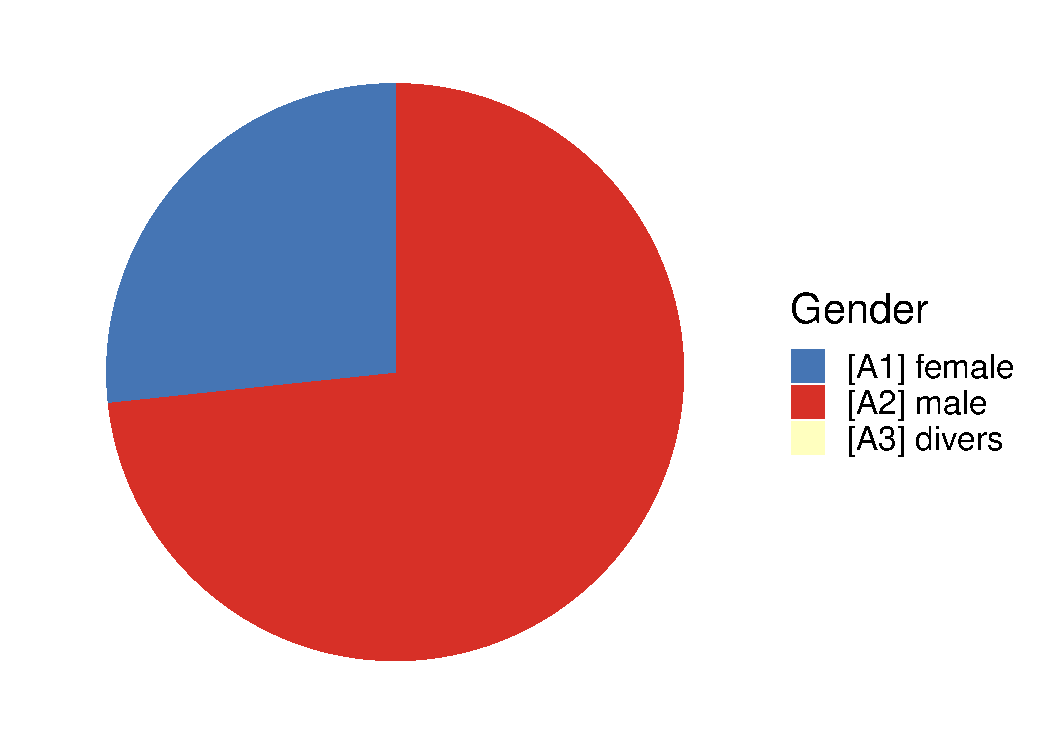
\includegraphics[width=\textwidth]{./appendices/gender}
	\caption{Geschlechterverteilung der Studienteilnehmer}
	\label{fig:gender}
\end{figure}

\begin{table*}
	\caption{Verteilung der Antworten zur Frage 'How much experience do you have with VR?'.}~\label{tab:sc_results_age}
	
	\setlength\tabcolsep{3pt}
	\renewcommand{\arraystretch}{1.4}% for the vertical padding
	\begin{tabularx}{\textwidth}{ | x || r | r | }
		\hline
		Studienfach 						& Absolutwerte 	& Prozentwerte \\ \hline\hline
		[A1] No experience at all 			& 10 			& 22.2\% \\ \hline
		[A2] Almost no experience 			& 15 			& 33.3\% \\ \hline
		[A3] Less than average experience 	& 3 			& 6.7\% \\ \hline
		[A4] Some experience 				& 10 			& 22.2\% \\ \hline
		[A5] More than average experience 	& 2 			& 4.4\% \\ \hline
		[A6] Experienced 					& 2 			& 4.4\% \\ \hline
		[A7] Very highly experienced 		& 3 			& 6.7\% \\ \hline
	\end{tabularx}
\end{table*}

\begin{table*}
	\caption{Verteilung der Antworten zur Frage 'How much experience do you have with AR?'.}~\label{tab:sc_results_age}
	
	\setlength\tabcolsep{3pt}
	\renewcommand{\arraystretch}{1.4}% for the vertical padding
	\begin{tabularx}{\textwidth}{ | x || r | r | }
		\hline
		Studienfach 						& Absolutwerte 	& Prozentwerte \\ \hline\hline
		[A1] No experience at all 			& 17 			& 37.7\% \\ \hline
		[A2] Almost no experience 			& 10 			& 22.2\% \\ \hline
		[A3] Less than average experience 	& 7 			& 15.5\% \\ \hline
		[A4] Some experience 				& 8 			& 17.7\% \\ \hline
		[A5] More than average experience 	& 2 			& 4.4\% \\ \hline
		[A6] Experienced 					& 1 			& 2.2\% \\ \hline
		[A7] Very highly experienced 		& 0 			& 0.0\% \\ \hline
	\end{tabularx}
\end{table*}

\begin{figure}
	% \centering
	\begin{subfigure}{0.48\textwidth}
		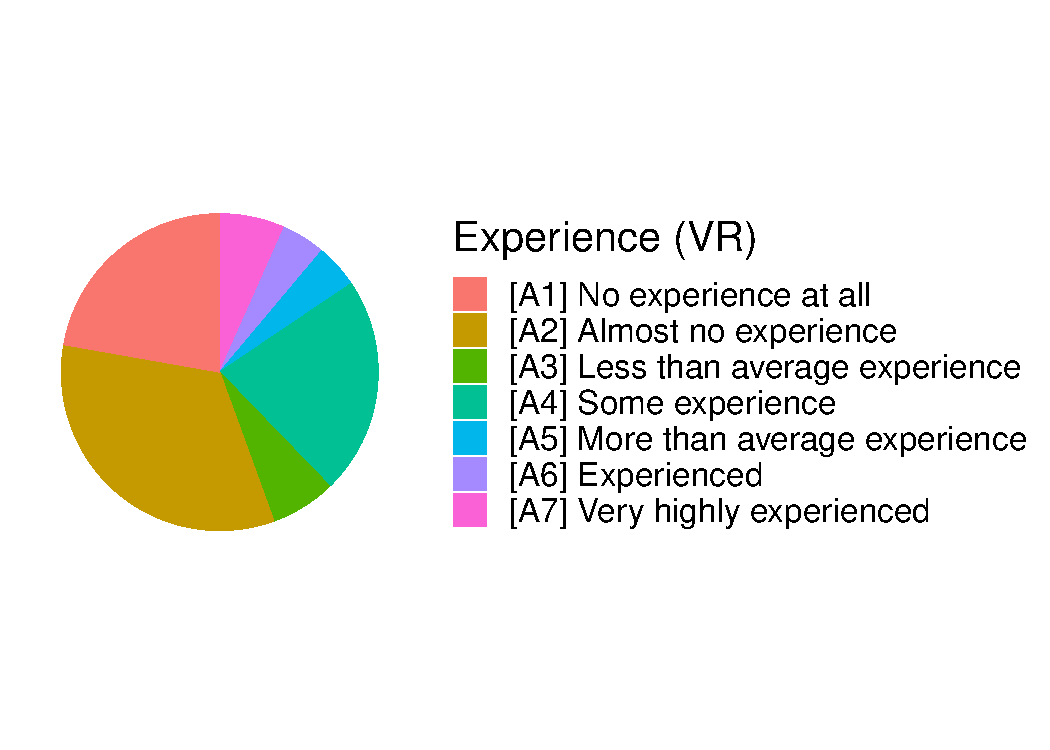
\includegraphics[width=\textwidth]{./appendices/expVr}
		\caption{Grafische Representation der Antworten zur Frage 'How much experience do you have with VR?'.}
		\label{fig:expVr}
	\end{subfigure}%
	\hfill
	\begin{subfigure}{0.48\textwidth}
		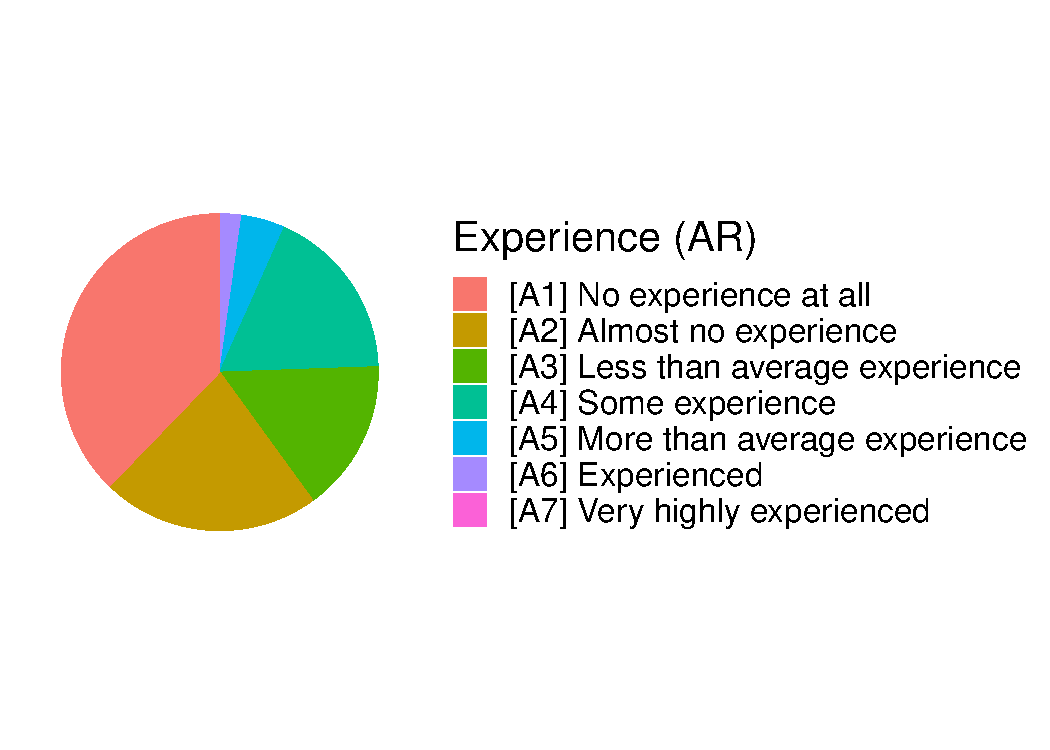
\includegraphics[width=\textwidth]{./appendices/expAr}
		\caption{Grafische Representation der Antworten zur Frage 'How much experience do you have with AR?'.}
		\label{fig:expAr}
	\end{subfigure}
	\caption{Erfahrungen mit virtueller und augmentierter Realität der Studienteilnehmer} % caption for whole figure
\end{figure}

\begin{table*}
	\caption{Verteilung der Antworten zur Frage 'What subject, if any, did you study or are you currently studying?'.}~\label{tab:sc_results_age}
	
	\setlength\tabcolsep{3pt}
	\renewcommand{\arraystretch}{1.4}% for the vertical padding
	\begin{tabularx}{\textwidth}{ | x || r | r | }
		\hline
		Studienfach & Absolutwerte & Prozentwerte \\ \hline\hline
		Biologie & 1 & 2.2\% \\ \hline
		Informatik & 8 & 17.8\% \\ \hline
		Informationssystemtechnik & 1 & 2.2\% \\ \hline
		Mathematik & 1 & 2.2\% \\ \hline
		Medieninformatik & 18 & 40\% \\ \hline
		Physik & 3 & 6.7\% \\ \hline
		Psychologie & 2 & 4.4\% \\ \hline
		Software Engineering & 8 & 17.8\% \\ \hline
		Wirtschaftsmathematik & 1 & 2.2\% \\ \hline
		Wirtschaftsphysik & 2 & 4.4\% \\ \hline
	\end{tabularx}
\end{table*}

\todoTob{Mehr Ergebnisse einfügen}
\todoAll{Ergebnisse (wertungsfrei) beschreiben}
